\section{Задание 1}

Создать HTML-страницу, которая при загрузке запрашивает дату вашего рождения и выводит на страницу день недели, число, месяц и год этой даты. Для месяцев и дней недели организовать массивы.

\begin{center}
  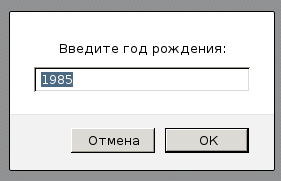
\includegraphics{img/Exercise_01/01.png}

  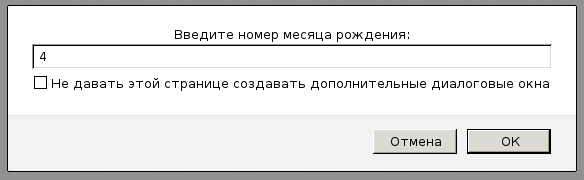
\includegraphics{img/Exercise_01/02.png}
  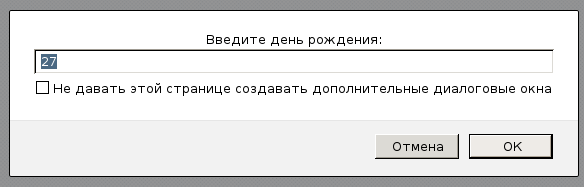
\includegraphics{img/Exercise_01/03.png}
  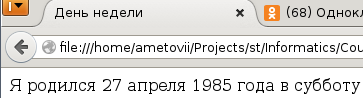
\includegraphics{img/Exercise_01/04.png}
\end{center}

Исходный код \verb|exercise_01.html|:

\begin{verbatim}
<!doctype html>
<html>
  <head>
    <title>День недели</title>
    <meta charset='utf-8' />
  </head>
  <body>
    <script>
      var birthYear=prompt("Введите год рождения:", "1985");
      var birthMonth=prompt("Введите номер месяца рождения:", "4");
      var birthDay=prompt("Введите день рождения:", "27");
      var birthDate=new Date();
      birthDate.setFullYear(birthYear);
      birthDate.setMonth(birthMonth-1);
      birthDate.setDate(birthDay);
      var monthes = ["января", "февраля",
                     "марта", "апреля",
                     "мая", "июня",
                     "июля", "августа",
                     "сентября", "октября",
                     "ноября", "декабря"];
      var weekDays = ["воскресенье", "понедельник",
		      "вторник", "среду",
		      "четверг", "пятницу",
		      "субботу"];
      document.write("Я родился "+birthDate.getDate()+
		     " "+monthes[birthDate.getMonth()]+
		     " "+birthDate.getFullYear()+" года в "+
		     weekDays[birthDate.getDay()]);
    </script>
  </body>
</html>
\end{verbatim}
